% 微波铁磁共振实验说明
\begin{figure}[htbp]
	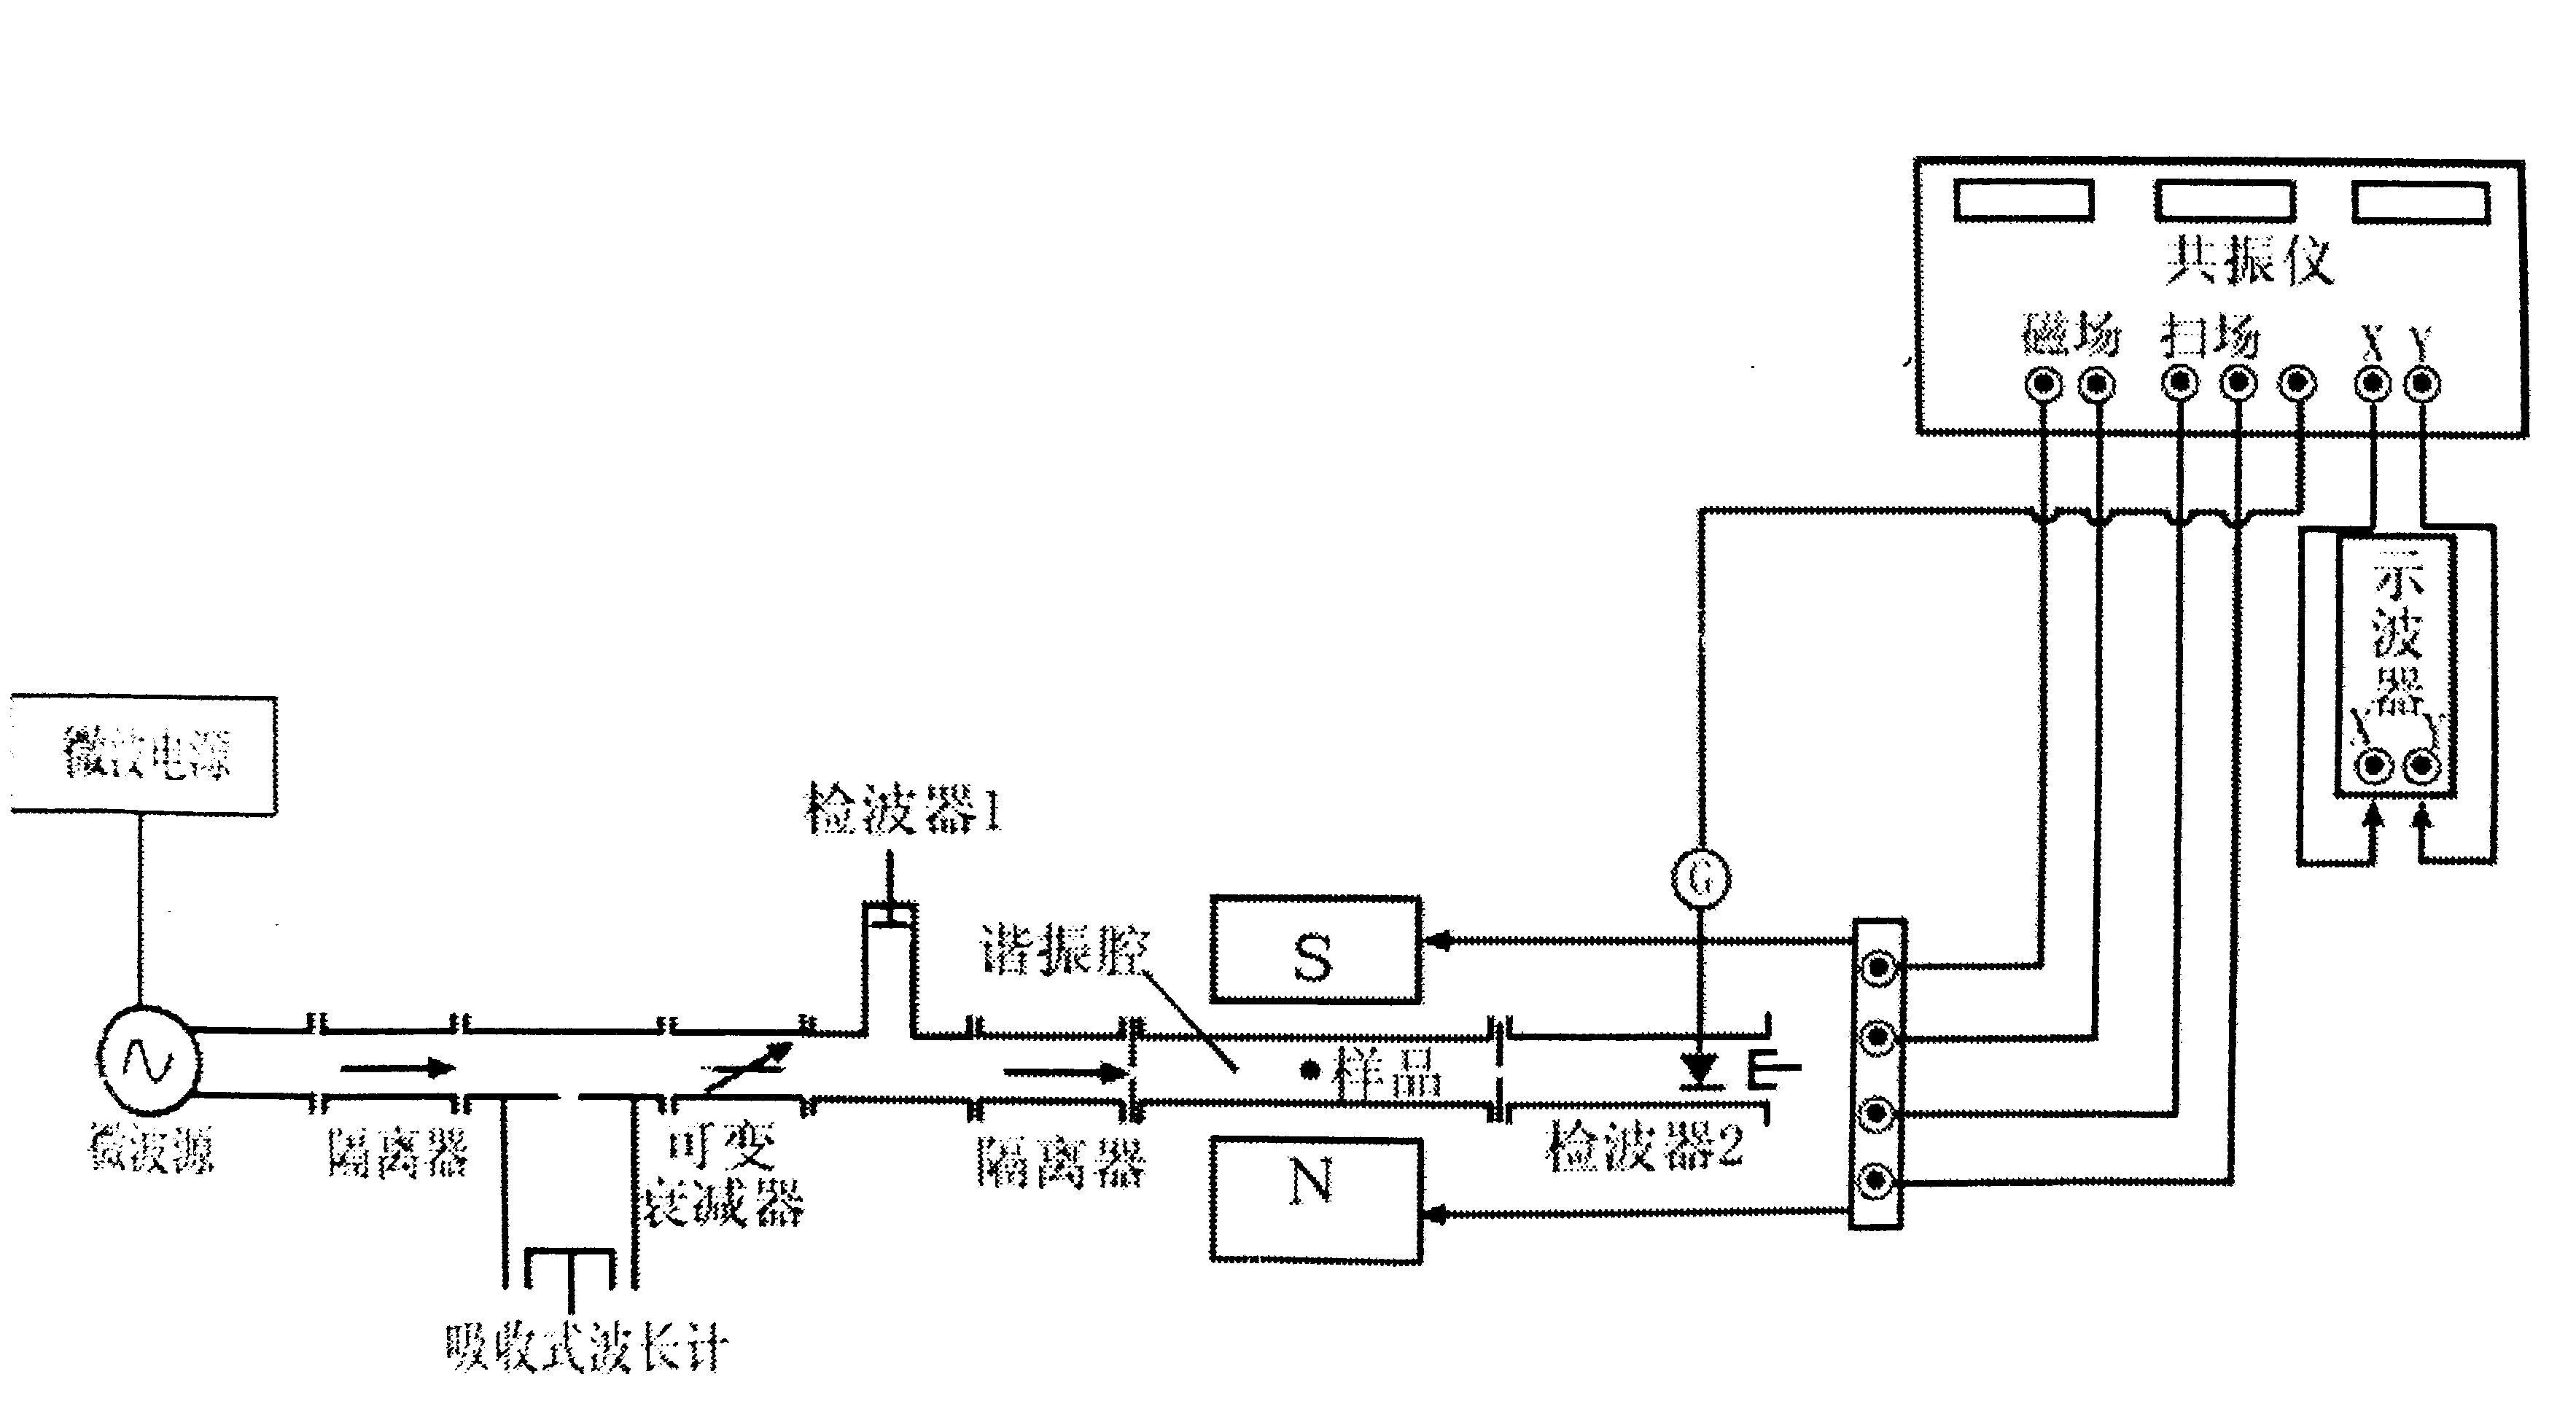
\includegraphics[width=.8\textwidth]{fig/scan/ExperimentalopticalpathdiagramofTransmissionresonatorFerromagneticresonanceExperiment.png}
	\caption{传输式谐振腔铁磁共振实验光路图\label{fig:传输式谐振腔铁磁共振实验光路图}}
\end{figure}
\begin{enumerate}
	\item 体效应微波振荡器工作曲线测量及性能测量
		\begin{enumerate}
			\item 打开体效应微波振荡器总电源,调节“频率"旋钮使频率读数位于9.000GHz 左右,预热至少30分钟。按\cref{fig:传输式谐振腔铁磁共振实验光路图}所示光路图检查光路是否连接妥当。
			\item 按下微波源信号的“等幅"和“教学"工作钮,在0$\sim$13V的电压范围内连续改变体效应管的主作电压,记录相应的工作电流值,画出体效应管在0$\sim$13V区间电流·电压曲线。利用光路中的吸收式波长计和检波器1测量工作电压在10$\sim$13V区间频率-电压曲线,分析体效应管的负阻区和微波工作区的电压范围。
			\item 弹起“教学"工作钮,此时体效应管工作在标准电压12.0V左右。调节体效应管功率钮和微波衰减器,使与检波器1连接的微安表的示数合适,调节频率旋钮,改变微波的频率范围(8.9GHz-9.2GHz),测量不同频率下的微波输出功率。\\
			注意,每次改变频率后,检波器要调谐。
		\end{enumerate}
	\item 铁磁共振实验
		\begin{enumerate}
			\item 检查传输式谐振腔中的金属耦合片是否装上。
			\item 本实验是在3厘米微波波段进行的,传输式谐振腔采用TEI。p矩型谐振腔(本 实验中$p$=8, $a$=2.295cm,$l$=19.30cm),样品采用直径大约为1-2mm的多晶或单晶铁氧体小球。电磁铁提供的外磁场强度为0$\sim$0.5T。根据{\color{red} ref 讲义公式(9)和(10)}估算谐振腔的谐振频率。
			\item 检测电磁铁电钮旋钮是否为最小,然后打开共振仪电源,工作方式设为检波。根据预习中对理论谐振频率的计算结果,在该频率附近连续调节微波频率,观察共振仪上的检波示数的变化,当表头示数发生变化时,及时调整检波器2的调谐活塞和灵敏度,使检波指针示数合适。观察示数随微波频率的变化关系。
			\item 仔细调节微波频率观察谐振腔的输出功率,找到其谐振频率$f_0$,将检波器2连接到微安电流表上,调节衰减器,使微安表示数合适,在此频率左右单调、逐点测量传输式谐振腔的谐振曲线,并计算其品质因数。
			\item 将微波频率设置为$f_0$,工作方式设为扫场,放入铁磁样品,调节磁场电流扫场为最大,调节磁场电流,直到在示波器(x-y扫描方式)观察到共振曲线,调节相移钮,使左右信号重合,调节各参数(电磁铁电流/相移/微调谐振频率),使共振曲线接近理想图形。
			\item 分别观察不同铁氧体样品的共振线宽。
			\begin{enumerate}
			\item 在谐振腔中放入不同的铁氧体样品,观察共振信号的变化,记录共振曲线的图像,分析不同样品共振信号的差异与成因。
			\item 用逐点法测量样品的共振曲线:
				\begin{enumerate}
					\item 将待测样品放入谐振腔,铁磁共振仪设为扫场方式,调节磁场电流,在示波器上观察样品的共振特征;
					\item 铁磁共振仪设为检波,将检波器2连接到微安表上,从小到大调节磁场电流,用逐点法测量样品的共振曲线,注意合理设置测量点的步长,测量前一定要使谐振腔调谐,使曲线左右远离共振时的信号功率尽量相等(如果共振曲线左右功率不等,应微调谐振频率),绘制$P-B$图,测量多晶样品的共振线宽$\Delta B$。
				\end{enumerate}
			\end{enumerate}
			\item 用高斯计测量电磁铁电流与磁场强度的关系。
			\item 计算样品的旋磁比$\gamma=\dfrac{B_0}{\omega_0}$、$g$因子和弛豫时间$\tau$。 
			\item 比较分析不同样品的弛豫时间不同的原因。
		\end{enumerate}
	\item 关机:将铁磁共振仪的电磁铁电流调至最小,关仪器电源开关。
\end{enumerate}